\section{Ejercicio 1: Una nueva esperanza}

    % Describir detalladamente el problema a resolver dando ejemplos del mismo
    % y sus soluciones.
    \subsection{Descripción del problema}

    \begin{figure}[ht]
        \begin{center}
            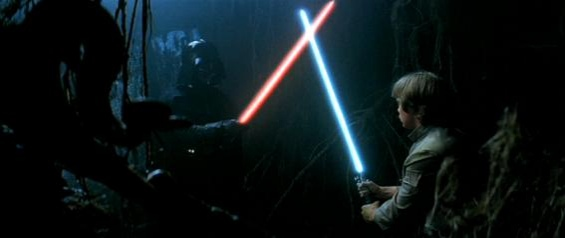
\includegraphics[width=10cm]{imagenes/una_nueva_esperanza.jpg}
            \caption*{``Ese lugar... es fuerte con el lado oscuro de la Fuerza. Un
            dominio del mal es. Dentro tú debes ir''.}
        \end{center}
    \end{figure}

    Como parte de su entrenamiento con el maestro Yoda, Luke Skywalker debe
    recorrer un complejo sistema que consta de $N$ cuevas, conectadas por $M$
    pasadizos. Cada pasadizo une dos cuevas entre sí, formando una red en la
    que siempre existe una forma de llegar desde una cueva hasta cualquier
    otra. Además, no todos los pasadizos son iguales: algunos de ellos son
    especiales, y para atravesarlos Luke deberá enfrentarse a sus mayores
    miedos. Recorrer cualquier pasadizo le demanda a Luke exactamente un
    minuto.

    Partiendo de una cueva etiquetada con el número $0$, Luke debe llegar en
    el menor tiempo posible a la cueva número $N-1$, donde lo espera Yoda.
    Sin embargo, su entrenamiento no estará completo hasta no haber pasado al
    menos por dos pasadizos especiales. Está permitido recorrer el mismo
    pasadizo más de una vez.

    Se pide implementar un algoritmo que determine el menor tiempo posible que
    le demandará a Luke completar su entrenamiento, y la secuencia de cuevas
    que deberá recorrer para lograrlo, con una complejidad temporal de
    $\ord(N + M)$.

    \vspace{1.25em}

    \textbf{Formato de entrada}: La primera línea consta de un entero positivo
    \texttt{N}, que indica la cantidad de cuevas, y un entero positivo
    \texttt{M}, que indica la cantidad de pasadizos. A continuación de esta
    línea siguen \texttt{M} líneas con enteros \texttt{Ai}, \texttt{Bi} y
    \texttt{Ei}, cada una de ellas correspondiente a un pasadizo, donde
    \texttt{Ai} y \texttt{Bi} son enteros (entre $0$ y $N-1$ inclusive) que
    indican los extremos del mismo, mientras que \texttt{Ei} indica
    el tipo de pasadizo ($0$ para los pasadizos comunes y $1$ para los
    especiales). Es decir, el formato de la entrada es el siguiente:

    \begin{verbatim}
    N M
    A0 B0 E0
    A1 B1 E1
    ...
    AM-1 BM-1 EM-1\end{verbatim}

    \vspace{.8em}

    \textbf{Formato de salida}: Debe devolverse una primera línea conteniendo
    la cantidad de minutos (\texttt{T}) que durará el entrenamiento de Luke,
    y una segunda línea con la lista ordenada de las cuevas (\texttt{I1},
    \texttt{I2}, \dots, \texttt{I(T-1)}) que deberá recorrer para
    completarlo, omitiendo la salida desde la cueva $0$ y la llegada a la
    cueva $N-1$. El formato requerido es el siguiente:

    \begin{verbatim}
    T
    I1 I2 ... I(T-1)\end{verbatim}

    \vspace{.8em}

    A continuación se incluyen, a modo de ejemplo, una posible entrada y una
    salida correcta para la misma:

    \vspace{.5em}
    \begin{tabular}{l @{\hskip 4em} l}
    \textbf{Entrada} & \textbf{Salida} \\
    \texttt{5 6}     & \texttt{3}      \\
    \texttt{0 1 0}   & \texttt{2 3}    \\
    \texttt{0 2 1}   &                 \\
    \texttt{0 4 0}   &                 \\
    \texttt{1 3 0}   &                 \\
    \texttt{2 3 0}   &                 \\
    \texttt{3 4 1}   &                 \\
    \end{tabular}
    \vspace{.5em}

    Es importante observar que puede haber más de una salida distinta válida.

    % Explicar de forma clara, sencilla, estructurada y concisa, las ideas
    % desarrolladas para la resolución del problema. Utilizar pseudocódigo y
    % lenguaje coloquial (no código fuente). Justificar por qué el
    % procedimiento resuelve efectivamente el problema.
    \subsection{Solución propuesta}

	\subsubsection{Modelo}

	Para resolver este problema se exigía encontrar el camino que recorriera al
	menos 2 pasillos especiales con un costo mínimo de tiempo, donde el mismo se
	define como el total de pasillos atravesados. Lo primero que se realizó fue
	modelar el problema con grafos dado que el mismo tenía características que
	sugerían que para la resolución iba a ser necesario calcular un camino mínimo de algún tipo.

	La primer idea de representación con grafos fue tener las cuevas como nodos y
	los pasillos como aristas. Sin embargo, quedaban aquí sin contemplar los
	pasillos especiales. Para subsanar esto, cada arista contiene además una bandera
	indicando si es o no un pasillo especial.

	Este grafo era una forma de modelar el problema donde aún no quedaba claro
	cómo resolver el ejercicio. Si se buscaba el camino mínimo del punto inicial
	al resto de las cuevas no existía ninguna garantía de que se cumpliera la
	condición de haber recorrido al menos 2 pasillos especiales.

	Para la versión final del modelo, lo que se hizo fue generar copias del
	grafo descrito anteriormente, teniendo como diferencia entre estos su
	\emph{estado}. El estado lo que indicará es para cada una de estas copias la
	cantidad de caminos especiales recorridos.

	Se tienen tres grafos, uno para cada uno de los siguientes estados:

	\begin{enumerate}
		\item{No se recorrió ningún pasillo especial.}
		\item{Se recorrió un pasillo especial.}
		\item{Se recorrieron al menos dos pasillos especiales.}
	\end{enumerate}

	\begin{figure}[H]
		\centering
		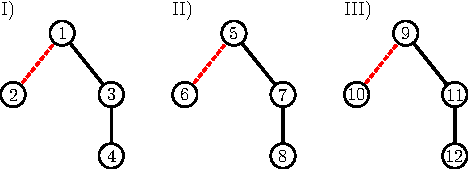
\includegraphics{imagenes/ej1_modelo_1.pdf}
		\caption{Visualización de los grafos con las aristas rojas representando un pasillo especial.}
		\label{ej1:fig_1}
	\end{figure}

	Una posible observación es que por más que cada grafo representa el mismo
	conjunto de cuevas y pasillos, para cada estado se utilizan
	números distintos para identificar cada nodo. Esto se debe a que ésta será
	la forma de identificar en qué estado se encuentra cada nodo. Se define la
	siguiente función donde $V$ es el número de nodo y $N$ el total de cuevas
	dado por la entrada:

	\begin{equation*}
		estado(V) =
		\begin{cases}
			1 & , V \leq N \\
			2 & , N < V \leq 2 * N \\
			3 & , 2 * N < V \leq 3 * N
		\end{cases}
	\end{equation*}

	Teniendo esta representación, se procede a explicar el algoritmo y
	solución desarrollada. Existen dos objetivos: que Luke atraviese al menos 2
	caminos especiales, que el camino que tome para lograr eso sea mínimo. Para
	lo segundo, como las aristas no poseen pesos, se puede utilizar
	\emph{Breadth First Search}, que permite obtener la distancia de un nodo
	cualquiera hacia el resto. Sin embargo esto solo no alcanza, ya que es
	requisito el recorrer al menos 2 caminos especiales. Para cumplir con esta
	condición se introduce una ligera modificación al \emph{BFS}: si un vecino
	se accede cruzando un pasillo especial, el nodo correspondiente en el estado
	siguiente se marca como visitado y se encolan sus vecinos.

	De esta manera lo que se logra es que en cuanto se realiza un cambio de
	estado (el salto a un vecino mediante un pasillo especial), se permite que
	el \emph{BFS} recorra cuevas que ya había visitado, con la diferencia de que
	cuenta con el hecho de que atravesó al menos un pasillo especial.

	Siguiendo esta lógica se obtiene la distancia de una cueva al resto en
	alguno de sus posibles estados. En particular, tomando el grafo
	correspondiente al estado donde se recorrieron al menos 2 pasillos
	especiales, la distancia hasta el nodo que equivale al $N - 1$ es la del camino mínimo
	pedido por el enunciado.

	A continuación se presenta el efecto de cada iteración del algoritmo sobre el grafo
	presentado en la Figura \ref{ej1:fig_1}:

	\begin{figure}[H]
		\centering
		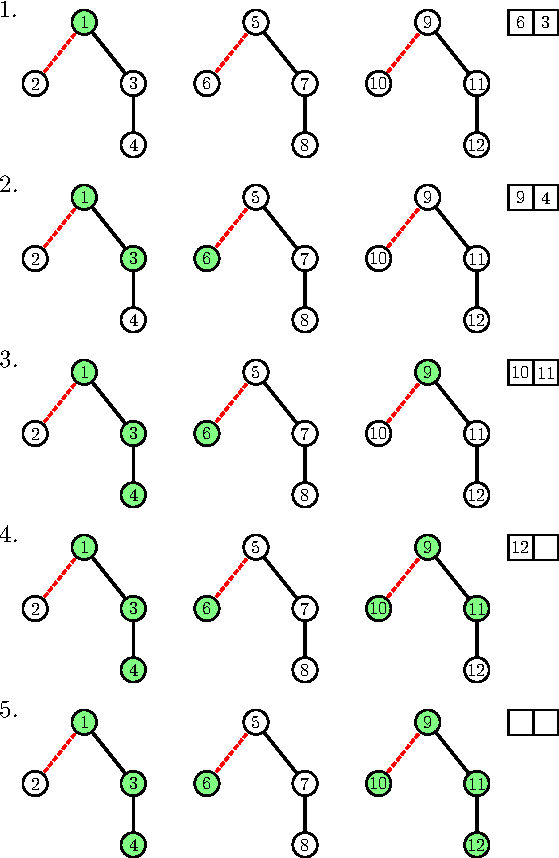
\includegraphics{imagenes/ej1_modelo_2.pdf}
		\caption{Visualización del \emph{BFS} marcando con verde los nodos
		visitados y el estado de la cola.}
		\label{ej1:bfs}
	\end{figure}

	Esta ejecución genera el siguiente árbol de caminos mínimos, donde se puede
	observar que se obtiene la distancia al nodo 12 que es el equivalente al $N
	- 1$ en el grafo donde se recorrieron al menos 2 pasillos especiales:

	\begin{figure}[H]
		\centering
		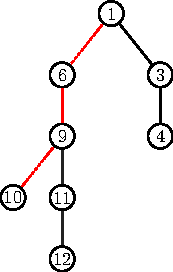
\includegraphics{imagenes/ej1_modelo_3.pdf}
		\caption{Árbol de caminos mínimos del nodo inicial al resto.}
	\end{figure}

	Una vez que se tiene este árbol de caminos mínimos, para armar la solución se trepa
	desde el nodo $N - 1$ (con $estado(N - 1) = 3$) hasta la
	raiz, traduciendo el índice de cada nodo al de su equivalente en el grafo
	original. Por ejemplo, el nodo 12 es en realidad la cueva 4 con $estado(12) =
	3$, por lo tanto a la hora de armar el camino se lo traducirá a 4.

    A continuación se exhibe el pseudocódigo del algoritmo que resuelve el problema:

    \begin{algorithm}
        \caption{BFS modificado}
        \label{algo:bfs}

        \Input{Un entero $N$ y un grafo $G$ de $N$ nodos y $M$ aristas, dado por un vector de
        listas de adyacencia}
        \Output{El camino mínimo entre el nodo 0 y el $N - 1$, pasando por al menos dos
        pasadizos especiales, dado como una pila de enteros}
        $predecesores$ $\gets$ vector de longitud $3N$ con cada valor en $sinPadre$ \;
        $colaNodos$ $\gets$ cola de enteros vacía \;
        $predecesores$[$0$] $\gets$ $0$ \;
        $colaNodos$.encolar($0$) \;

        \While{$colaNodos$ no esté vacía} {
            $nodo$ $\gets$ $colaNodos$.desencolar() \;
            $nodoEfectivo$ $\gets$ índice real de $nodo$ \;
            \ForEach{vecino $v$ de $nodoEfectivo$}{
                $nodoAdyacente$ $\gets$ $v$ + diferencia de estado entre $nodo$ y $nodoEfectivo$ \;
                \If{hay camino especial entre $nodoEfectivo$ y $v$} {
                    cambiar de estado a $nodoAdyacente$, tiene un camino especial mas \;
                }
                \If{$predecesores$[$nodoAdyacente$] == $sinPadre$} {
                    $predecesores$[$nodoAdyacente$] $\gets$ $nodo$ \;
                    $colaNodos$.encolar($nodoAdyacente$) \;
                }
            }
        }

        $caminoOptimo$ $\gets$ pila de enteros vacía \;
        $actual$ $\gets$ nodo $N - 1$ con estado $alMenosDosCaminosEspeciales$ \;
        \While{$actual$ sea distinto del nodo 0} {
            $caminoOptimo$.apilar(indice real de $actual$) \;
            $actual$ $\gets$ $predecesores$[$actual$] \;
        }
        \Return{$predecesores$}
    \end{algorithm}

	Habiendo introducido la idea detrás de la solución desarrolada, se procede a
	demostrar que esto efectivamente funciona, es decir que con esta
	modificación al \emph{BFS} siempre se encontrará un camino mínimo hasta la
	cueva $N - 1$ habiendo recorrido al menos 2 pasillos especiales.

	\subsubsection{Demostración de correctitud}

	Para probar que se cumple lo pedido, primero se realizará inducción sobre los ciclos
	del \emph{BFS} modificado buscando demostrar que al finalizar, se obtienen
	los caminos mínimos teniendo en cuenta la condición de pasadizos especiales
	recorridos.

	\subsubsection*{Correctitud del ciclo}

	El invariante a demostrar será el siguiente: al terminar el ciclo $k$ del
	\emph{BFS} modificado se obtienen todos los nodos a distancia a lo sumo $k$
	del inicial en alguno de los estados posibles y ninguno más. Esto se probará
	mediante inducción en los ciclos del algoritmo.

	~

	\textbf{Caso base: } $k = 1$

	En el caso base se tiene únicamente el nodo inicial marcado como
	visitado con distancia 0. Como se trata del nodo inicial, se encuentra en el primer estado ya que
	no se recorrieron pasadizos especiales. Por lo tanto, existen dos posibles
	formas de accionar con respecto a sus vecinos:

	\begin{enumerate}
		\item{
			El vecino está conectado mediante un pasadizo común, con lo cual en
			el grafo del nodo inicial se lo marca con distancia 1 y encolan sus
			vecinos.
		}
		\item{
			El vecino está conectado mediante un pasadizo especial, por lo tanto
			en el grafo en el estado siguiente, es decir en el que se cuenta con
			que se recorrió un pasadizo especial, se lo marca con distancia 1 y
			encolan sus vecinos.
		}
	\end{enumerate}

	De esta forma una vez finalizada la iteración $k = 1$ se obtienen todos los
	nodos que están a distancia 1 del nodo inicial en uno de los dos estados
	posibles.

	~

	\textbf{Paso inductivo: } $k > 1$

	Como hipótesis inductiva se cuenta con que vale el invariante para $k - 1$,
	por lo tanto se tiene la distancia para todos los nodos a lo sumo
	a distancia $k - 1$ para alguno de los estados descritos y además se
	tienen encolados para visitar los que están a distancia $k$ (no así los que
	se encuentran a distancia mayor o igual a $k + 1$).

	Ahora acá existen distintas posibilidades por el hecho de que a diferencia
	del caso base, los nodos encolados no tienen por qué necesariamente
	encontrarse en el primer estado. Pueden haber nodos pertenecientes al
	segundo como tercer estado (un pasadizo especial o al menos dos recorridos).

	Es entonces necesario probar que en cada caso el invariante seguirá
	valiendo:

	\begin{enumerate}
		\item{
			El nodo encolado pertenece al primer estado. En este escenario, al
			igual que con el caso base existen dos posibles formas de operar en
			función de si se accede a un vecino mediante una arista especial:

			\begin{enumerate}
				\item{
					El vecino está conectado mediante un pasadizo común, con lo
					cual en el grafo del primer estado se observa si ya se
					encuentra marcado. En caso de no estar marcado, como
					proviene de un nodo a distancia $k - 1$, en ese mismo grafo
					se le asigna la distancia $k$ y encolan sus vecinos.
				}
				\item{
					El vecino está conectado mediante un pasadizo especial, con
					lo cual en el grafo del segundo estado se observa si ya se
					encuentra marcado. En caso de no estar marcado, como
					proviene de un nodo a distancia $k - 1$, en ese mismo
					grafo se le asigna la distancia $k$ y encolan sus vecinos.
				}
			\end{enumerate}
		}
		\item{
			El nodo encolado pertenece al segundo estado. Nuevamente existen dos
			posibles formas de operar en función de si la arista que lo conecta
			a un vecino es especial:

			\begin{enumerate}
				\item{
					El vecino está conectado mediante un pasadizo común, con lo
					cual en el grafo del segundo estado se observa si ya se
					encuentra marcado. En caso de no estar marcado, como
					proviene de un nodo a distancia $k - 1$, en ese mismo
					grafo se le asigna la distancia $k$ y encolan sus vecinos.
				}
				\item{
					El vecino está conectado mediante un pasadizo especial, con
					lo cual en el grafo del tercer estado se observa si ya se
					encuentra marcado. En caso de no estar marcado, como
					proviene de un nodo a distancia $k - 1$, en ese mismo
					grafo se le asigna la distancia $k$ y encolan sus vecinos.
				}
			\end{enumerate}
		}
		\item{
			Por último, en caso de que el nodo encolado pertenezca al tercer
			estado existe una única manera de proceder, ya que en caso de que un
			vecino se encuentre conectado mediante una arista especial ya no hay
			un estado sucesor.

			Si en el grafo del tercer estado alguno de los vecinos no se
			encuentra marcado, como proviene de un nodo a distancia $k - 1$, se
			le asigna distancia $k$ y es encolado para ser visitado.
		}
	\end{enumerate}

	Habiendo contemplado cada escenario posible es posible afirmar que al
	finalizar la iteración $k$ con $k > 2$ se obtienen todos los nodos a
	distancia $k$ para alguno de los estados posibles.

	Por inducción en los ciclos del algoritmo, se demuestra que para
	toda iteración se cumple el invariante, con lo cual al finalizar se obtiene
	la distancia de todos los nodos para alguno de los estados descritos y
	ninguno más.

	Queda probar entonces que si existe al menos una arista especial entonces
	siempre se obtendrá la distancia hasta el nodo $N - 1$ en el tercer estado,
	es decir el mínimo camino tal que se atraviesan al menos dos caminos
	especiales.

	Para probar que esto vale, se demostrará que el grafo vinculado al tercer
	estado, tendrá todos sus nodos marcados con su respectiva distancia.

	\subsubsection*{Existencia de un camino mínimo al nodo $N - 1$ en el tercer
	estado}

	Como se dijo previamente, se probará que todo nodo perteneciente al tercer
	estado se encuentra marcado con su respectiva distancia. Supongamos que esto
	no es cierto, que existe al menos un nodo sin marcar o con un valor que no
	es su distancia. Esto podría ser resultado de uno de los siguientes
	escenarios:

	\begin{itemize}
		\item{
			Existe al menos un nodo sin marcar
			\begin{itemize}
				\item{Nunca se salta al tercer estado, en este caso resultando en que no
					haya ningún nodo marcado en el mismo.}
				\item{Se llega al tercer estado pero no se recorren todos sus nodos.}
			\end{itemize}
		}
		\item{
			Existe al menos un nodo cuyo valor no representa su distancia al
			nodo inicial
			\begin{itemize}
				\item{Tiene un valor mayor o menor a la distancia.}
			\end{itemize}
		}
	\end{itemize}

	\underline{Existe al menos un nodo sin marcar}

	Si se considera el primer escenario, esto implica que jamás se saltó del
	segundo al tercer estado. Sin embargo para que esto ocurriese se debería
	cumplir una de las siguientes condiciones: jamás se saltó al segundo estado
	o ningún nodo del segundo estado tiene un vecino conectado mediante una
	arista especial. Es fácil ver que ninguna de estas condiciones se cumplen.

	La primera, como se asume que siempre existe al menos un pasadizo especial,
	por el comportamiento del \emph{BFS} modificado eventualmente se
	encontrará un nodo cuyo vecino está conectado por una arista especial y en el
	grafo del segundo estado este vecino no estará marcado, con lo cual lo
	marcará y encolará sus vecinos saltando de esta forma al segundo estado.

	Lo segundo, que ningún nodo del segundo estado tenga un vecino conectado
	mediante un pasadizo especial, carece de sentido por el hecho de que el
	grafo vinculado con el segundo estado es una copia del primero. Entonces, si
	del primero se salta al segundo, en este estado el nodo seguro tendrá como
	vecino el nodo del que saltó, también conectado mediante una arista
	especial.

	Por lo tanto habiendo visto que ninguna de estas condiciones se cumplen
	queda demostrado que el primer escenario nunca puede suceder, ya que si se
	llega al segundo estado y además se cuenta con que habrán vecinos conectados
	mediante aristas especiales esto significa que van a existir saltos al
	tercer estado.

	Queda entonces el segundo escenario, se llega al tercer estado pero no se
	recorren todos sus nodos. Esto es algo que podría suceder en el primer o
	segundo estado (véase Figura \ref{ej1:bfs}) pero no en el tercero.

	Si quedan nodos sin marcar en el tercer grafo es porque los mismos jamás
	fueron encolados para visitarlos. Ya se demostró que al tercer estado se
	salta en algún momento, con lo cual al menos uno de los nodos de
	seguro va a estar marcado. Luego por la descripción del \emph{BFS}
	modificado tenemos que un nodo en el tercer estado ya no salta a otro grafo,
	con lo cual todos los vecinos no marcados son visitados. De esta forma no
	hay manera que queden nodos sin visitar, ya que o bien están marcados de
	forma directa como vecinos de un nodo del segundo estado, o son alcanzados por
	el avance del \emph{BFS} de alguno de los nodos provenientes de un salto del segundo estado.

	\underline{Existe al menos un nodo cuyo valor no representa su distancia al nodo inicial}

	Si hay un nodos con valor distinto a su distancia existen dos casos
	a contemplar: que el mismo sea mayor o menor.

	Para ambos escenarios se estaría rompiendo el invariante del \emph{BFS}
	modificado. Si el valor del nodo es mayor o menor entonces en
	la iteración $k$ correspondiente a la distancia se procedió de forma
	incorrecta asignándole un valor distinto de $k$. Como se demostró que vale el
	invariante, no es posible que esto ocurra.

	Así se prueba entonces que ninguno de los escenarios planteados pueden
	suceder, con lo cual todos los nodos en el tercer estado están marcados y
	poseen un camino mínimo hasta el nodo inicial en el primer estado. Como
	consecuencia de esto, en particular de seguro existe un camino mínimo del
	nodo incial en el primer estado al nodo $N - 1$ en el tercer estado.

    % Deducir una cota de complejidad temporal del algoritmo propuesto (en
    % función de los parámetros que se consideren correctos) y justificar por
    % qué el algoritmo la cumple. Utilizar el modelo uniforme.
    \subsection{Complejidad teórica}
    Crear el vector de representación para los estados de los nodos tiene un
	costo de $\ord(3N)$.

	En el peor caso, el \emph{BFS} va a marcar todos los nodos en cada estado
	posible. Este escenario implica que para cada nodo en todos sus posibles
	estados tendrá que consultar si alguno de sus vecinos se encuentra o no
	marcado. Esto resulta en la suma de los grados de todos los nodos:

	\begin{equation*}
		\ord(\sum_{i=1}^{n=3 N} d(v_i)) = \ord(2 \times 3M) = \ord(6M)
	\end{equation*}

	Por último se arma el camino óptimo trepando del nodo destino $N - 1$ en el
	tercer estado hasta el nodo origen en estado inicial. Esto en el peor caso
	resulta en un camino con $3N$ nodos, que es la longitud del mayor camino
	simple posible. Por lo tanto para la construcción del camino óptimo se
	tiene $\ord(3N)$.

	La complejidad total queda $\ord(6N + 6M) = \ord(N + M)$ donde al ser el
	grafo conexo se cumple que $M \geq N - 1$, con lo cual la cota final resulta $\ord(M)$.

    % Realizar experimentación para medir la performance, usando un conjunto
    % de casos de test que permitan observar los tiempos de ejecución en
    % función de los parámetros de entrada, tanto para instancias aleatorias
    % (detallando cómo fueron generadas) como para instancias particulares
    % (peor/mejor caso, por ejemplo). Presentar en forma gráfica una
    % comparación entre los tiempos medidos y la complejidad teórica y extraer
    % conclusiones.
    \subsection{Experimentación}

    Una vez completada la implementación de la solución, se llevaron a cabo
    pruebas experimentales con el objetivo de verificar que se cumpliera la
    cota teórica prevista para la complejidad asintótica de $\ord(M)$, siendo
    $M$ la cantidad de aristas del grafo tomado como entrada.

    Las pruebas realizadas pueden dividirse en dos grupos. Por un lado, se
    midió el tiempo de ejecución para diferentes familias de instancias
    generadas de forma aleatoria, para corroborar así que en todas ellas la
    complejidad mostrara el comportamiento previsto. Por otra parte, se
    llevaron a cabo pruebas soporte de las anteriores, para confirmar
    hipótesis acerca de la relación entre el rendimiento temporal del
    algoritmo y la modificación de ciertas variables de los datos de entrada.

    \subsubsection{Experimentos principales}

    \newcommand\constante{300}

    Se construyeron generadores de escenarios de prueba aleatorios para distintas
    instancias del problema, permitiendo modificar el parámetro $M$, es decir,
    la cantidad de aristas de los grafos generados. Se procuró que las familias
    de grafos generadas para cada escenario resultaran \emph{coherentes}, en
    el sentido de que se intentó que la complejidad de su resolución dependiera
    solo de la cantidad de aristas y no de otros factores inherentes a su
    construcción.

    Un factor que resultó especialmente complejo fue la distribución de las
    aristas especiales en los grafos generados. Se decidió, entre las alternativas
    posibles, generar a los grafos con una proporción fija $p$ de aristas
    especiales sobre el total de aristas, elegidas al azar; es decir, durante
    la generación de las instancias, cada arista que se agrega se marca como
    especial con una probabilidad de $p$. De esta manera se intenta
    homogeneizar las instancias tanto como sea posible. En las pruebas
    adicionales, se experimenta con el efecto que tienen diversos valores de
    $p$ sobre el tiempo de ejecución del algoritmo; en estas pruebas, se
    utilizó un valor fijo de $p = 0.3$.

    A continuación se detallan las características de los distintos escenarios
    generados, junto con la notación utilizada en los gráficos para referirse
    a los mismos.
    \begin{itemize}
        \item $T_r$: Árboles generados de forma aleatoria. Para cada valor de
        $M$, se genera un grafo de $N = M+1$ nodos. A continuación, se van
        agregando aristas al grafo de forma aleatoria, asegurándose de que no
        se formen ciclos, hasta completar $M$ aristas. La metodología para
        hacerlo es similar al algoritmo de Prim: en cada paso se elige al azar
        un nodo que ya forme parte del árbol y uno que no, y se los conecta
        por medio de una arista.
        \item $T_i$: Árboles generados de forma incremental. Para el primer
        valor de $M$ considerado, se genera un árbol según la metodología
        anterior. Para los valores de $M$ siguientes, se considera el grafo
        generado para el valor previo, completándolo a $M+1$ nodos y agregando
        aristas de forma aleatoria hasta formar un nuevo árbol con $M$
        aristas.
        \item $K$: Grafo completo. Para cada valor de $M$ se considera un
        grafo completo. Del hecho de que un grafo completo de $N$ nodos tiene
        $M = \frac{N \times (N - 1)}{2}$ aristas, se deduce que un grafo
        completo de $M$ aristas deberá tener $\frac{1 + \sqrt{1 + 8 \times
        M}}{2}$ nodos. Los valores de $M$ considerados se aproximan de forma
        tal que el resultado de esta fórmula sea un número entero. En este
        caso, al igual que en los dos siguientes, el elemento de azar se
        reduce a la selección del subconjunto de aristas especiales.
        \item $P$: Camino simple de $M$ aristas, cuyos extremos son los nodos
        $0$ y $N-1$.
        \item $A$: Árbol $M$-ario completo de $M$ aristas. Se construye un
        árbol donde el nodo $0$ resulta adyacente a todos los demás.
    \end{itemize}

    Cabe destacar que el escenario $K$ tiene una cantidad de nodos
    considerablemente menor que todos los demás (del orden de $\sqrt{M}$
    frente a $M$), lo cual hace esperable que su tiempo de ejecución resulte
    también relativamente menor. No obstante, los escenarios $P$ y $A$
    podrían verse favorecidos por la simpleza de su resolución. Los dos
    escenarios con árboles aleatorios ($T_r$ y $T_i$) parecen ser los que
    presentan un mayor desafío desde el punto de vista computacional, debido a
    su gran cantidad de nodos y su morfología compleja.

    En la Figura \ref{fig:exp1:var-m-base} pueden observarse los resultados
    del tiempo de ejecución observado para todos los escenarios, considerando
    valores de $M$ entre $20000$ y $800000$. Se ilustra también la cota
    teórica mediante una función lineal $c \times M$; el valor de $c$
    utilizado es $\constante$.

    \begin{figure}[H]
        \centering
        \caption{Tiempos de ejecución según la cantidad de aristas
        ($c=\constante$)}
        \label{fig:exp1:var-m-base}
        \begin{tikzpicture}
            \begin{axis}[
                    title={},
                    xlabel={Tamaño de entrada ($M$)},
                    ylabel={Tiempo de ejecución (nanosegundos)},
                    scaled x ticks=false,
                    scaled y ticks=false,
                    enlargelimits=0.05,
                    width=0.5\textwidth,
                    height=0.5\textwidth,
                    legend pos=outer north east,
                    legend cell align=left,
                    xmin=1
                ]
                \addplot[color=darkgray]
                    table[x index=0, y expr={x*\constante}]
                    {../exp/UnaNuevaEsperanza-varM-arboles};
                \addplot[color=red]
                    table[x index=0,y index=1]
                    {../exp/UnaNuevaEsperanza-varM-inc-arboles};
                \addplot[color=orange]
                    table[x index=0,y index=1]
                    {../exp/UnaNuevaEsperanza-varM-arboles};
                \addplot[color=green]
                    table[x index=0,y index=1]
                    {../exp/UnaNuevaEsperanza-varM-completos};
                \addplot[color=blue]
                    table[x index=0,y index=1]
                    {../exp/UnaNuevaEsperanza-varM-caminos};
                \addplot[color=violet]
                    table[x index=0,y index=1]
                    {../exp/UnaNuevaEsperanza-varM-m-arios};
                \legend{$c \times M$, $T_{T_i}$, $T_{T_r}$, $T_{K}$, $T_{P}$,
                $T_{A}$}
            \end{axis}
        \end{tikzpicture}
    \end{figure}

    En la Figura \ref{fig:exp1:var-m-div-const} se ilustra el resultado de
    dividir todos los tiempos observados por su correspondiente valor de $M$.
    Puede notarse claramente que el crecimiento de todas las funciones
    observadas queda acotado por la constante $c$, corroborando en forma
    empírica la complejidad de $\ord(M)$ estimada en forma teórica.

    Se observa que los escenarios $A$ y $P$ presentan un rendimiento
    superior al escenario $K$, incluso aunque sus instancias cuentan con una
    mayor cantidad de nodos. A continuación se exponen hipótesis acerca de
    las razones por las que esto pudo haber ocurrido. En el caso $A$, dado que
    todos los nodos están unidos al nodo $0$, son encolados todos juntos en
    una misma iteración, reduciendo la cantidad total de veces que debe
    repetirse el procedimiento. El caso $P$, por su parte, se ve favorecido
    porque desde cada nodo puede visitarse un único vecino. Si la arista que
    lo une con dicho vecino resulta ser especial, la primera ``copia'' del
    grafo será abandonada definitivamente (todos los nodos siguientes
    estarán automáticamente en el estado ``\emph{se recorrió un pasillo
    especial}''), evitando una gran cantidad de iteraciones sobre los
    mismos.

    Un detalle a destacar es que el escenario $T_i$ presentó un rendimiento
    notablemente inferior al del escenario $T_r$, pese a que \emph{a priori}
    las instancias consideradas para ambos casos parecen ser similares. Una
    hipótesis posible es que el método de construcción de los árboles $T_r$
    incrementa la probabilidad de que la distancia entre los nodos $0$ y
    $N-1$ sea baja, y que esto repercute positivamente en el desempeño del
    algoritmo. No obstante, sería necesario realizar experimentos adicionales
    y analizar con mucho más detalle el comportamiento de estas instancias
    para corroborar la validez de esta hipótesis.

    \begin{figure}[H]
        \centering
        \caption{Cociente entre tiempo de ejecución y tamaño de la instancia
        ($c=\constante$)}
        \label{fig:exp1:var-m-div-const}
        \begin{tikzpicture}
            \begin{axis}[
                    title={},
                    xlabel={Tamaño de entrada ($M$)},
                    ylabel={Tiempo de ejecución (nanosegundos)},
                    scaled x ticks=false,
                    scaled y ticks=false,
                    enlargelimits=0.05,
                    width=0.5\textwidth,
                    height=0.5\textwidth,
                    legend pos=outer north east,
                    legend cell align=left,
                    xmin=1
                ]
                \addplot[color=darkgray]
                    table[x index=0, y expr={\constante}]
                    {../exp/UnaNuevaEsperanza-varM-arboles};
                \addplot[color=red]
                    table[x index=0,y expr={\thisrowno{1} / x}]
                    {../exp/UnaNuevaEsperanza-varM-inc-arboles};
                \addplot[color=orange]
                    table[x index=0,y expr={\thisrowno{1} / x}]
                    {../exp/UnaNuevaEsperanza-varM-arboles};
                \addplot[color=green]
                    table[x index=0,y expr={\thisrowno{1} / x}]
                    {../exp/UnaNuevaEsperanza-varM-completos};
                \addplot[color=blue]
                    table[x index=0,y expr={\thisrowno{1} / x}]
                    {../exp/UnaNuevaEsperanza-varM-caminos};
                \addplot[color=violet]
                    table[x index=0,y expr={\thisrowno{1} / x}]
                    {../exp/UnaNuevaEsperanza-varM-m-arios};
                \legend{$c$, $T_{A_i}/M$, $T_{A_r}/M$, $T_{C}/M$, $T_{P}/M$, $T_{K}/M$}
            \end{axis}
        \end{tikzpicture}
    \end{figure}

    \subsubsection{Experimentos adicionales}

    Como se mencionó anteriormente, una de las cualidades deseables en las
    familias de grafos elegidas para realizar los experimentos es que la
    complejidad de su resolución no se vea afectada por variables externas al
    experimento y que resulten imposibles de controlar. Esto resulta
    especialmente difícil de verificar en el caso de las instancias generadas
    de forma totalmente aleatoria, como sucede con el escenario $T_r$. Es por
    esto que se decidió realizar, en forma complementaria, una prueba
    experimental para corroborar que diferentes grafos generados de esta forma
    no produjeran tiempos de ejecución excesivamente diferentes para idénticos
    valores de $M$.

    Para esto, se seleccionaron cuatro valores de $M$, $100000$, $2000000$,
    $400000$ y $800000$, y para todos ellos se generaron $200$ grafos
    distintos utilizando los procedimientos aleatorios antes descriptos, para
    los escenarios $T_r$ y $K$. Así, se logró verificar que las instancias
    generadas para estos escenarios se comportan de una forma uniforme,
    validando su utilización en el experimento anterior.

    La Figura \ref{fig:exp1:aleatorios-arb} muestra los resultados obtenidos
    para el escenario $T_r$ (árboles), mientras que la Figura
    \ref{fig:exp1:aleatorios-comp} hace lo propio con el escenario $K$
    (grafos completos).

    \begin{figure}[H]
        \centering
        \caption{Tiempos de ejecución para árboles generados en forma
        aleatoria}
        \label{fig:exp1:aleatorios-arb}
        \begin{tikzpicture}
            \begin{axis}[
                    title={},
                    mark size=1pt,
                    xlabel={Número de instancia},
                    ylabel={Tiempo de ejecución (nanosegundos)},
                    scaled x ticks=false,
                    scaled y ticks=false,
                    enlargelimits=0.05,
                    width=0.5\textwidth,
                    height=0.5\textwidth,
                    legend pos=outer north east,
                    legend cell align=left,
                    xmin=1
                ]
                \addplot[color=blue,only marks]
                    table[x expr=\coordindex, y index=1]
                    {../exp/UnaNuevaEsperanza-aleatorios-arb-m100k};
                \addplot[color=green,only marks]
                    table[x expr=\coordindex, y index=1]
                    {../exp/UnaNuevaEsperanza-aleatorios-arb-m200k};
                \addplot[color=orange,only marks]
                    table[x expr=\coordindex, y index=1]
                    {../exp/UnaNuevaEsperanza-aleatorios-arb-m400k};
                \addplot[color=red,only marks]
                    table[x expr=\coordindex,y index=1]
                    {../exp/UnaNuevaEsperanza-aleatorios-arb-m800k};
                \legend{$M = 100000$, $M = 200000$, $M = 400000$, $M = 800000$}
            \end{axis}
        \end{tikzpicture}
    \end{figure}

    \begin{figure}[H]
        \centering
        \caption{Tiempos de ejecución para grafos completos generados en forma
        aleatoria}
        \label{fig:exp1:aleatorios-comp}
        \begin{tikzpicture}
            \begin{axis}[
                    title={},
                    mark size=1pt,
                    xlabel={Número de instancia},
                    ylabel={Tiempo de ejecución (nanosegundos)},
                    scaled x ticks=false,
                    scaled y ticks=false,
                    enlargelimits=0.05,
                    width=0.5\textwidth,
                    height=0.5\textwidth,
                    legend pos=outer north east,
                    legend cell align=left,
                    xmin=1
                ]
                \addplot[color=blue,only marks]
                    table[x expr=\coordindex, y index=1]
                    {../exp/UnaNuevaEsperanza-aleatorios-comp-m100k};
                \addplot[color=green,only marks]
                    table[x expr=\coordindex, y index=1]
                    {../exp/UnaNuevaEsperanza-aleatorios-comp-m200k};
                \addplot[color=orange,only marks]
                    table[x expr=\coordindex, y index=1]
                    {../exp/UnaNuevaEsperanza-aleatorios-comp-m400k};
                \addplot[color=red,only marks]
                    table[x expr=\coordindex,y index=1]
                    {../exp/UnaNuevaEsperanza-aleatorios-comp-m800k};
                \legend{$M = 100000$, $M = 200000$, $M = 400000$, $M = 800000$}
            \end{axis}
        \end{tikzpicture}
    \end{figure}

    Resulta interesante observar cómo la dispersión en el caso del escenario
    $K$ parece ser menor que la presente en el escenario $T_r$. Es razonable
    pensar que esto se debe a que, durante la generación de las instancias
    para este último escenario, el azar juega un rol considerablemente más
    importante.

    Otra de las decisiones que se tomó durante los experimentos anteriores fue
    fijar en $0.3$ la proporción del total de aristas que serían marcadas como
    especiales. Esto generó dudas acerca del efecto que produciría una
    variación de este valor en el rendimiento temporal del algoritmo,
    si se mantuvieran estáticos los demás parámetros.

    Con esta motivación, se realizaron pruebas con dos valores distintos de
    $M$ ($200000$ y $400000$) y los mismos dos escenarios del experimento
    anterior ($T_r$ y $K$), haciendo variar la proporción $p$ de aristas
    especiales dentro del intervalo $(0, 1]$. La Figura
    \ref{fig:exp1:aristas-esp} expone los tiempos de ejecución observados.

    \begin{figure}[H]
        \centering
        \caption{Tiempos de ejecución en función de la proporción de aristas
        especiales}
        \label{fig:exp1:aristas-esp}
        \begin{tikzpicture}
            \begin{axis}[
                    title={},
                    xlabel={Proporción de aristas especiales ($p$)},
                    ylabel={Tiempo de ejecución (nanosegundos)},
                    scaled x ticks=false,
                    scaled y ticks=false,
                    width=0.5\textwidth,
                    height=0.5\textwidth,
                    legend pos=north east,
                    legend cell align=left,
                ]
                \addplot[color=red]
                    table[x index=0,y index=1]
                    {../exp/UnaNuevaEsperanza-aristas-esp-arb-m200k};
                \addplot[color=blue]
                    table[x index=0,y index=1]
                    {../exp/UnaNuevaEsperanza-aristas-esp-comp-m200k};
                \addplot[color=red]
                    table[x index=0,y index=1]
                    {../exp/UnaNuevaEsperanza-aristas-esp-arb-m400k};
                \addplot[color=blue]
                    table[x index=0,y index=1]
                    {../exp/UnaNuevaEsperanza-aristas-esp-comp-m400k};
                \legend{$T_{T_r}$ (Árboles aleatorios), $T_K$ (Grafos completos)}
            \end{axis}
        \end{tikzpicture}
    \end{figure}

    Se observa claramente que los tiempos de ejecución son considerablemente
    más altos para valores bajos de $p$, es decir, cuando las aristas
    especiales son escasas. Esto resulta razonable teniendo en cuenta que
    una alta densidad de aristas especiales hace que el algoritmo pase
    rápidamente a las nuevas ``copias'' del grafo, evitando tener que iterar
    sobre gran parte de los nodos hasta encontrar las mismas. También se
    observa, no obstante, que el valor óptimo para esta proporción se
    encuentra en todos los casos aproximadamente entre $0.2$ y $0.3$,
    notándose en los tiempos de ejecución una ligera tendencia a empeorar para
    valores mayores. Si bien queda fuera de los límites del alcance de
    este trabajo, podría resultar de interés profundizar a futuro la
    experimentación para determinar las causas de este fenómeno.
